\documentclass{article}
\usepackage{amsfonts} % For open face letters
\usepackage{amsmath} % For align*
\usepackage{graphicx} % For images
\usepackage{enumitem} % For customisable list labels
\usepackage{siunitx} % For units
\graphicspath{{./images/}}

\renewcommand{\vec}[1]{\boldsymbol{\mathbf{#1}}}
\newcommand{\dvec}[1]{\dot{\vec{#1}}}
\newcommand{\ddvec}[1]{\ddot{\vec{#1}}}
\newcommand{\uvec}[1]{\hat{\vec{#1}}}

\newcommand{\ke}{\frac{1}{4 \pi \epsilon_0}}

\def\rcurs{{\mbox{$\resizebox{.09in}{.08in}{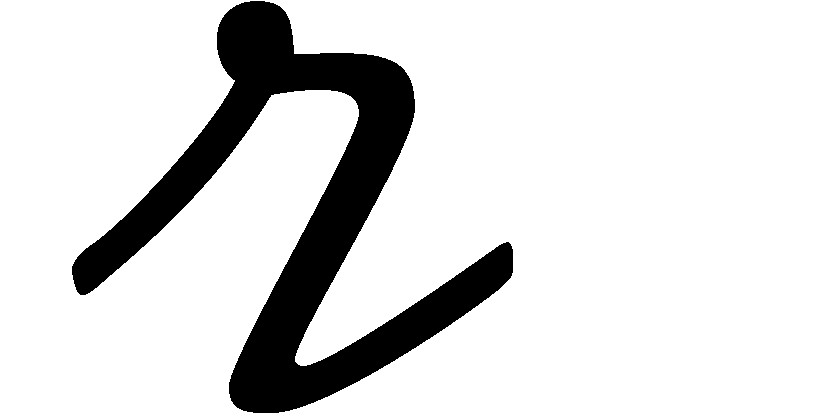
\includegraphics[trim= 1em 0 14em 0,clip]{ScriptR}}$}}}
\def\brcurs{{\mbox{$\resizebox{.09in}{.08in}{
\includegraphics[trim= 1em 0 14em 0,clip]{BoldR}}$}}}
\def\hrcurs{{\mbox{$\hat \brcurs$}}}

\setlist[enumerate, 1]{label={(\alph*)}}
\setlist[enumerate, 2]{label={(\roman*)}}

\title{Introduction to Electrodynamics by David J. Griffiths Problems}
\author{Chris Doble}
\date{December 2023}

\begin{document}

\maketitle

\tableofcontents

\setcounter{section}{1}
\section{Electrostatics}

\subsection{}

\begin{enumerate}
  \item $\vec{0}$

  \item The same as if only the opposite charge were present — all others are cancelled out.
\end{enumerate}

\subsection{}

\begin{align*}
  \vec{E} & = \ke 2 \frac{q}{\rcurs^2} \cos \theta \uvec{x}      \\
          & = \ke \frac{d q}{[(d / 2)^2 + z^2]^{3 / 2}} \uvec{x}
\end{align*}

\subsection{}

\begin{align*}
  \vec{r}  & = z \uvec{z}                                                                                                                          \\
  \vec{r}' & = x \uvec{x}                                                                                                                          \\
  \brcurs  & = z \uvec{z} - x \uvec{x}                                                                                                             \\
  \rcurs   & = \sqrt{x^2 + z^2}                                                                                                                    \\
  \hrcurs  & = \frac{z \uvec{z} - x \uvec{x}}{\sqrt{x^2 + z^2}}                                                                                    \\
  \vec{E}  & = \ke \int_0^L \frac{\lambda}{x^2 + z^2} \frac{z \uvec{z} - x \uvec{x}}{\sqrt{x^2 + z^2}} \,d x                                       \\
           & = \ke \lambda \left( z \uvec{z} \int_0^L \frac{1}{(x^2 + z^2)^{3 / 2}} \,d x - \uvec{x} \int_0^L \frac{x}{(x^2 + z^2)} \,d x \right)  \\
           & = \ke \lambda \left[ \frac{L}{z \sqrt{L^2 + z^2}} \uvec{z} - \left( \frac{1}{z} - \frac{1}{\sqrt{L^2 + z^2}} \right) \uvec{x} \right] \\
           & = \ke \frac{\lambda}{z} \left[ \left( -1 + \frac{z}{\sqrt{L^2 + z^2}} \right) \uvec{x} + \frac{L}{\sqrt{L^2 + z^2}} \uvec{z} \right]
\end{align*}

\subsection{}

The electric field a distance $z$ above the midpoint of a line segment of length $2 L$ and uniform line charge $\lambda$ is \[\vec{E} = \ke \frac{2 \lambda L}{z \sqrt{z^2 + L^2}} \uvec{z}.\]

Applying this to the four sides of the square, the horizontal components of opposite sides cancel leaving only the vertical component.

\begin{align*}
  \cos \theta & = \frac{z}{\rcurs}                                                                                                      \\
              & = \frac{z}{\sqrt{(a / 2)^2 + z^2}}                                                                                      \\
  \vec{E}     & = 4 \left( \ke \frac{\lambda a}{\sqrt{(a / 2)^2 + z^2} \sqrt{(a / 2)^2 + (a / 2)^2 + z^2}} \uvec{z} \right) \cos \theta \\
              & = \ke \frac{4 a \lambda z}{[(a / 2)^2 + z^2] \sqrt{(a^2 / 2) + z^2}} \uvec{z}
\end{align*}

\subsection{}

\begin{align*}
  \vec{E} & = \ke \int_0^{2 \pi} \frac{\lambda r}{r^2 + z^2} \cos \alpha \,d \theta \,\uvec{z} \\
          & = \ke \frac{2 \pi \lambda r z}{(r^2 + z^2)^{3 / 2}} \uvec{z}
\end{align*}

\subsection{}

\begin{align*}
  \vec{E} & = \ke \int \frac{d q}{\rcurs^2} \cos \theta \uvec{z}                                                          \\
          & = \ke \int_0^{2 \pi} \int_0^R \frac{\sigma}{r^2 + z^2} \frac{z}{\sqrt{r^2 + z^2}} r \,d r \,d \theta \uvec{z} \\
          & = \ke 2 \pi \sigma z \int_0^R \frac{r}{(r^2 + z^2)^{3 / 2}} \,d r \,\uvec{z}                                  \\
          & = \ke 2 \pi \sigma z \left( \frac{1}{z} - \frac{1}{\sqrt{R^2 + z^2}} \right) \uvec{z}
\end{align*}

When $R \rightarrow \infty$ \[\vec{E} = \frac{\sigma}{2 \epsilon_0} \uvec{z}.\]

\subsection{}

\[\vec{E} = \begin{cases}
    \ke \frac{q}{z^2} \uvec{z} & z > R \\
    \vec{0}                    & z < R
  \end{cases}\]

\subsection{}

\[\vec{E} = \begin{cases}
    \ke \frac{q}{z^2} \uvec{z}   & z > R \\
    \ke \frac{q z}{R^3} \uvec{z} & z < R
  \end{cases}\]

\subsection{}

\begin{enumerate}
  \item

        \begin{align*}
          \rho & = \epsilon_0 \nabla \cdot \vec{E}                              \\
               & = \epsilon_0 \frac{1}{r^2} \frac{\partial}{\partial r} (k r^5) \\
               & = 5 \epsilon_0 k r^2
        \end{align*}

  \item

        \begin{align*}
          Q_\text{enc} & = \epsilon_0 \oint \vec{E} \cdot d \vec{a}                                                        \\
                       & = \epsilon_0 \int_0^{2 \pi} \int_0^\pi k R^3 R \,d \theta R \sin \theta \,d \phi                  \\
                       & = 2 \pi \epsilon_0 k R^5 [-\cos \theta]_0^\pi                                                     \\
                       & = 4 \pi \epsilon_0 k R^5                                                                          \\
          Q_\text{enc} & = \int_V \rho \,d \tau                                                                            \\
                       & = \int_0^{2 \pi} \int_0^\pi \int_0^R 5 \epsilon_0 k r^2 \,d r r \,d \theta r \sin \theta \,d \phi \\
                       & = 10 \pi \epsilon_0 k \int_0^\pi \int_0^R r^4 \sin \theta \,d r \,d \theta                        \\
                       & = 2 \pi \epsilon_0 k R^5 [-\cos \theta]_0^\pi                                                     \\
                       & = 4 \pi \epsilon_0 k R^5
        \end{align*}
\end{enumerate}

\subsection{}

If the charge was surrounded by $8$ such cubes the total flux through all the cubes would be $q / \epsilon_0$. There are $24$ outside faces to the larger cube, so the total flux through the shaded face is $q / (24 \epsilon_0)$.

\subsection{}

\begin{align*}
  \int \vec{E}_\text{inside} \cdot d \vec{a}  & = \frac{Q_\text{enc}}{\epsilon_0}     \\
                                              & = 0                                   \\
  \vec{E}_\text{inside}                       & = \vec{0}                             \\
  \int \vec{E}_\text{outside} \cdot d \vec{a} & = \frac{Q_\text{enc}}{\epsilon_0}     \\
  4 \pi r^2 E_\text{outside}                  & = \frac{4 \pi R^2 \sigma}{\epsilon_0} \\
  \vec{E}_\text{outside}                      & = \ke \frac{q}{r^2} \uvec{r}
\end{align*}

\subsection{}

\begin{align*}
  \int \vec{E} \cdot d \vec{a} & = \frac{Q_\text{enc}}{\epsilon_0}             \\
  4 \pi r^2 E                  & = \frac{\frac{4}{3} \pi r^3 \rho}{\epsilon_0} \\
  \vec{E}                      & = \frac{r \rho}{3 \epsilon_0} \uvec{r}
\end{align*}

\subsection{}

\begin{align*}
  \int \vec{E} \cdot d \vec{a} & = \frac{Q_\text{enc}}{\epsilon_0}                       \\
  2 \pi s l E                  & = \frac{l \lambda}{\epsilon_0}                          \\
  \vec{E}                      & = \frac{1}{2 \pi \epsilon_0} \frac{\lambda}{s} \uvec{s}
\end{align*}

\subsection{}

\begin{align*}
  Q_\text{enc}                 & = \int_V \rho \,d \tau                                                             \\
                               & = \int_0^{2 \pi} \int_0^\pi \int_0^r k r'^3 \sin \theta \,d r' \,d \theta \,d \phi \\
                               & = 2 \pi k \int_0^\pi \left[ \frac{1}{4} r'^4 \sin \theta \right]_0^r \,d \theta    \\
                               & = \frac{1}{2} \pi k r^4 [-\cos \theta]_0^\pi                                       \\
                               & = \pi k r^4                                                                        \\
  \int \vec{E} \cdot d \vec{a} & = \frac{Q_\text{enc}}{\epsilon_0}                                                  \\
  4 \pi r^2 E                  & = \frac{\pi k r^4}{\epsilon_0}                                                     \\
  \vec{E}                      & = \frac{k r^2}{4 \epsilon_0} \uvec{r}
\end{align*}

\subsection{}

\begin{enumerate}
  \item $\vec{E} = \vec{0}$

  \item

        \begin{align*}
          Q_\text{enc} & = \int_0^{2 \pi} \int_0^\pi \int_a^r k \sin \theta \,d r' \,d \theta \,d \phi \\
                       & = 4 \pi k (r - a)                                                             \\
          4 \pi r^2 E  & = \frac{4 \pi k (r - a)}{\epsilon_0}                                          \\
          \vec{E}      & = \frac{k (r - a)}{\epsilon_0 r^2} \uvec{r}
        \end{align*}

  \item $\vec{E} = \frac{k (b - a)}{\epsilon_0 r^2} \uvec{r}$
\end{enumerate}

\subsection{}

\begin{enumerate}
  \item

        \begin{align*}
          Q_\text{enc} & = \pi s^2 l \rho                       \\
          2 \pi s l E  & = \frac{\pi s^2 l \rho}{\epsilon_0}    \\
          \vec{E}      & = \frac{s \rho}{2 \epsilon_0} \uvec{s}
        \end{align*}

  \item \[\vec{E} = \frac{a^2 \rho}{2 \epsilon_0 s} \uvec{s}\]

  \item \[\vec{E} = \vec{0}\]
\end{enumerate}

\subsection{}

\begin{align*}
  2 A E_\text{inside}   & = \frac{2 A y \rho}{\epsilon_0}           \\
  \vec{E}_\text{inside} & = \frac{y \rho}{\epsilon_0}               \\
  \vec{E}               & = \begin{cases}
                              \frac{d \rho}{\epsilon_0}  & d < y      \\
                              \frac{y \rho}{\epsilon_0}  & 0 < y < d  \\
                              -\frac{y \rho}{\epsilon_0} & -d < y < 0 \\
                              -\frac{d \rho}{\epsilon_0} & y < -d
                            \end{cases}
\end{align*}

\subsection{}

The electric field inside a uniformly charged solid sphere is \[\vec{E} = \frac{r \rho}{3 \epsilon_0} \uvec{r}.\]

\begin{align*}
  \vec{d} & = \vec{r}_1 - \vec{r}_2                                                               \\
  \vec{E} & = \frac{r_1 \rho}{3 \epsilon_0} \uvec{r}_1 - \frac{r_2 \rho}{3 \epsilon_0} \uvec{r}_2 \\
          & = \frac{\rho}{3 \epsilon_0} (\vec{r}_1 - \vec{r}_2)                                   \\
          & = \frac{\rho}{3 \epsilon_0} \vec{d}
\end{align*}

\setcounter{subsection}{19}
\subsection{}

a is impossible because its curl is nonzero.

\begin{align*}
  V         & = -\int_0^y 2 k x y' \,d y' - \int_0^z 2 k y z' \,d z                                    \\
            & = -2 k x \left[ \frac{1}{2} y'^2 \right]_0^y - 2 k y \left[ \frac{1}{2} z'^2 \right]_0^z \\
            & = -k (x y^2 + y z^2)                                                                     \\
  -\nabla V & = k [y^2 \uvec{x} + (2 x y + z^2) \uvec{y} + 2 y z \uvec{z}]                             \\
            & = \vec{E}
\end{align*}

\subsection{}

\begin{align*}
  \vec{E}                  & = \begin{cases}
                                 \ke \frac{q}{r^2}   & r > R \\
                                 \ke \frac{q r}{R^3} & r < R
                               \end{cases}                                                                    \\
  V_\text{outside}(r)      & = -\int_\infty^r \ke \frac{q}{r'^2} \,d r'                                                       \\
                           & = -\ke q \left[ -\frac{1}{r'} \right]_\infty^r                                                   \\
                           & = \ke \frac{q}{r}                                                                                \\
  -\nabla V_\text{outside} & = \ke \frac{q}{r^2} \uvec{r}                                                                     \\
                           & = \vec{E}_\text{outside}                                                                         \\
  V_\text{inside}(r)       & = -\left( \int_\infty^R \ke \frac{q}{r'^2} \,d r' + \int_R^r \ke \frac{q r'}{R^3} \,d r' \right) \\
                           & = -\left( -\ke \frac{q}{R} + \ke \frac{q}{R^3} \left[ \frac{1}{2} r'^2 \right]_R^r \right)       \\
                           & = \ke \frac{q}{2 R} \left[ 3 - \left( \frac{r}{R} \right)^2 \right]                              \\
  -\nabla V_\text{inside}  & = \ke \frac{q r}{R^3} \uvec{r}                                                                   \\
                           & = \vec{E}_\text{inside}
\end{align*}

\subsection{}

\begin{align*}
  \vec{E}   & = \frac{1}{2 \pi \epsilon_0} \frac{\lambda}{s} \uvec{s}          \\
  V         & = -\int_O^s \frac{1}{2 \pi \epsilon_0} \frac{\lambda}{s'} \,d s' \\
            & = -\frac{1}{2 \pi \epsilon_0} \lambda \ln \frac{s}{O}            \\
  -\nabla V & = \frac{1}{2 \pi \epsilon_0} \frac{\lambda}{s} \uvec{s}
\end{align*}

\subsection{}

\begin{align*}
  \vec{E} & = \begin{cases}
                \vec{0}                                   & r < a     \\
                \frac{k (r - a)}{\epsilon_0 r^2} \uvec{r} & a < r < b \\
                \frac{k (b - a)}{\epsilon_0 r^2} \uvec{r} & b < r
              \end{cases}                                                                                           \\
  V(0)    & = -\int_\infty^0 E \,d r                                                                                                                          \\
          & = -\left( \int_\infty^b \frac{k (b - a)}{\epsilon_0 r^2} \,d r + \int_b^a \frac{k (r - a)}{\epsilon_0 r^2} \,d r \right)                          \\
          & = -\left( \frac{k (b - a)}{\epsilon_0} \left[ -\frac{1}{r} \right]_\infty^b + \frac{k}{\epsilon_0} \left[ \ln r + \frac{a}{r} \right]_b^a \right) \\
          & = -\left[ -\frac{k (b - a)}{\epsilon_0 b} + \frac{k}{\epsilon_0} \left( \ln a + 1 - \ln b - \frac{a}{b} \right) \right]                           \\
          & = -\frac{k}{\epsilon_0} \left( -1 + \frac{a}{b} + \ln \frac{a}{b} + 1 - \frac{a}{b} \right)                                                       \\
          & = \frac{k}{\epsilon_0} \ln \frac{b}{a}
\end{align*}

\subsection{}

\begin{align*}
  V(b) - V(0) & = -\int_0^b E \,d r                                                                                                            \\
              & = -\left( \int_0^a \frac{s \rho}{2 \epsilon_0} \,d s + \int_a^b \frac{a^2 \rho}{2 \epsilon_0 s} \,d s \right)                  \\
              & = -\left( \frac{\rho}{2 \epsilon_0} \left[ \frac{1}{2} s^2 \right]_0^a + \frac{a^2 \rho}{2 \epsilon_0} \ln \frac{b}{a} \right) \\
              & = -\left( \frac{a^2 \rho}{4 \epsilon_0} + \frac{a^2 \rho}{2 \epsilon_0} \ln \frac{b}{a} \right)                                \\
              & = -\frac{a^2 \rho}{4 \epsilon_0} \left( 1 + 2 \ln \frac{a}{b} \right)
\end{align*}

\subsection{}

\begin{enumerate}
  \item \[V = \ke \frac{2 q}{\sqrt{(d / 2)^2 + z^2}}\]

  \item

        \begin{align*}
          V & = \ke \int_{-L}^L \frac{\lambda}{\sqrt{x^2 + z^2}} \,d x                    \\
            & = \ke \lambda \ln \left( 1 + \frac{2 L (L + \sqrt{L^2 + z^2})}{z^2} \right)
        \end{align*}

  \item

        \begin{align*}
          V & = \ke \int_0^{2 \pi} \int_0^R \frac{\sigma}{\sqrt{r^2 + z^2}} r \,d r \,d \theta \\
            & = \ke 2 \pi \sigma (\sqrt{R^2 + z^2} - z)
        \end{align*}
\end{enumerate}

\subsection{}

\begin{align*}
  V_\text{bottom}                & = \ke \int_0^{2 \pi} \int_0^h \frac{\sqrt{2} \sigma z}{\sqrt{2} z} \,d \phi \,d z             \\
                                 & = \frac{\sigma h}{2 \epsilon_0}                                                               \\
  V_\text{top}                   & = \ke \int_0^{2 \pi} \int_0^h \frac{\sqrt{2} \sigma z}{\sqrt{z^2 + (h - z)^2}} \,d \phi \,d z \\
                                 & = \frac{\sqrt{2} \sigma}{2 \epsilon_0} \int_0^h \frac{z}{\sqrt{z^2 + (h - z)^2}} \,d z        \\
                                 & = \frac{\sigma h}{4 \epsilon_0} \ln (3 + 2 \sqrt{2})                                          \\
  V_\text{bottom} - V_\text{top} & = \frac{\sigma h}{2 \epsilon_0} \left[ 1 - \frac{1}{2} \ln (3 + 2 \sqrt{2}) \right]           \\
\end{align*}

\setcounter{subsection}{27}
\subsection{}

\begin{align*}
  V(r) & = \ke \int_0^{2 \pi} \int_0^\pi \int_0^R \frac{\rho r'^2 \sin \theta}{\sqrt{r^2 + r'^2 - 2 r r' \cos \theta}} \,d r' \,d \theta \,d \phi \\
       & = \frac{\rho}{2 \epsilon_0} \int_0^\pi \int_0^R \frac{r'^2 \sin \theta}{\sqrt{r^2 + r'^2 - 2 r r' \cos \theta}} \,d r' \,d \theta        \\
       & = \frac{\rho}{2 \epsilon_0} \left( R^2 - \frac{r^2}{3} \right)                                                                           \\
       & = \frac{q}{8 \pi \epsilon_0 R} \left( 3 - \frac{r^2}{R^2} \right)
\end{align*}

\setcounter{subsection}{30}
\subsection{}

\begin{enumerate}
  \item \[W = \frac{q^2}{4 \pi \epsilon_0 a} \left( \frac{1}{\sqrt{2}} - 2 \right)\]

  \item

        \begin{align*}
          W & = \ke \left( -\frac{q^2}{a} + \frac{q^2}{\sqrt{2} a} - \frac{q^2}{a} - \frac{q^2}{a} + \frac{q^2}{\sqrt{2} a} - \frac{q^2}{a} \right) \\
            & = \frac{q^2}{2 \pi \epsilon_0 a} \left( \frac{1}{\sqrt{2}} - 2 \right)
        \end{align*}
\end{enumerate}

\subsection{}

\begin{align*}
  % Conservation of energy
  W                                            & = \ke \frac{q_A q_B}{a}                                                           \\
  W                                            & = K_1 + K_2                                                                       \\
  \ke \frac{q_A q_B}{a}                        & = \frac{1}{2} m_A v_A^2 + \frac{1}{2} m_B v_B^2                                   \\
  \frac{1}{2 \pi \epsilon_0} \frac{q_A q_B}{a} & = m_A v_A^2 + m_B v_B^2                                                           \\
  % Conservation of momentum
  0                                            & = m_B v_B - m_A v_A                                                               \\
  v_B                                          & = \frac{m_A}{m_B} v_A                                                             \\
  \frac{1}{2 \pi \epsilon_0} \frac{q_A q_B}{a} & = m_A v_A^2 + m_B \left( \frac{m_A}{m_B} v_A \right)^2                            \\
                                               & = m_A v_A^2 + \frac{m_A^2}{m_B} v_A^2                                             \\
                                               & = \frac{m_A (m_A + m_B)}{m_B} v_A^2                                               \\
  v_A                                          & = \sqrt{\frac{1}{2 \pi \epsilon_0} \frac{q_A q_B}{(m_A + m_B) a} \frac{m_B}{m_A}} \\
  v_B                                          & = \sqrt{\frac{1}{2 \pi \epsilon_0} \frac{q_A q_B}{(m_A + m_B) a} \frac{m_A}{m_B}}
\end{align*}

\subsection{}

\begin{align*}
  W & = \ke \left( -\frac{q^2}{a} + \frac{q^2}{2 a} - \frac{q^2}{3 a} + \ldots \right) \\
    & = \ke \frac{q^2}{a} \sum_{n = 1}^\infty \frac{(-1)^n}{n}                         \\
    & = -\ke \frac{q^2}{a} \ln 2
\end{align*}

\subsection{}

\begin{enumerate}
  \item

        \begin{align*}
          V & = \begin{cases}
                  \ke \frac{q}{2 R} \left[ 3 - \left( \frac{r}{R} \right)^2 \right] & r < R \\
                  \ke \frac{q}{r}                                                   & r > R
                \end{cases}                                                                                       \\
          W & = \frac{1}{2} \int \rho V \,d \tau                                                                                                                                \\
            & = \frac{1}{2} \int_0^{2 \pi} \int_0^\pi \int_0^R \rho \ke \frac{q}{2 R} \left[ 3 - \left( \frac{r}{R} \right)^2 \right] r^2 \sin \theta \,d r \,d \theta \,d \phi \\
            & = \frac{q \rho}{8 \epsilon_0 R} \int_0^\pi \int_0^R \left[ 3 - \left( \frac{r}{R} \right)^2 \right] r^2 \sin \theta \,d r \,d \theta                              \\
            & = \frac{q \rho R^2}{5 \epsilon_0}                                                                                                                                 \\
            & = \frac{q R^2}{5 \epsilon_0} \frac{q}{\frac{4}{3} \pi R^3}                                                                                                        \\
            & = \ke \frac{3 q^2}{5 R}
        \end{align*}

  \item

        \begin{align*}
          \vec{E} & = \begin{cases}
                        \ke \frac{q}{r^2} \uvec{r}   & r > R \\
                        \ke \frac{q r}{R^3} \uvec{r} & r < R
                      \end{cases}                                                                                                                                                                                 \\
          E^2     & = \begin{cases}
                        \frac{1}{16 \pi^2 \epsilon_0^2} \frac{q^2}{r^4}     & r > R \\
                        \frac{1}{16 \pi^2 \epsilon_0^2} \frac{q^2 r^2}{R^6} & r < R
                      \end{cases}                                                                                                                                                          \\
          W       & = \frac{\epsilon_0}{2} \int E^2 \,d \tau                                                                                                                                                                               \\
                  & = \frac{\epsilon_0}{2} \left( \int_0^{2 \pi} \int_0^\pi \int_0^R \frac{1}{16 \pi^2 \epsilon_0^2} \frac{q^2 r^2}{R^6} r^2 \sin \theta \,d r \,d \theta \,d \phi \right.                                                 \\
                  & \qquad \left. + \int_0^{2 \pi} \int_0^\pi \int_R^\infty \frac{1}{16 \pi^2 \epsilon_0^2} \frac{q^2}{r^4} r^2 \sin \theta \,d r \,d \theta \,d \phi \right)                                                              \\
                  & = \frac{\epsilon_0}{2} \frac{1}{16 \pi^2 \epsilon_0^2} 2 \pi q^2 \left( \int_0^\pi \int_0^R \frac{r^4}{R^6} \sin \theta \,d r \,d \theta + \int_0^\pi \int_R^\infty \frac{1}{r^2} \sin \theta \,d r \,d \theta \right) \\
                  & = \frac{1}{16 \pi \epsilon_0} q^2 \left( \int_0^\pi \int_0^R \frac{r^4}{R^6} \sin \theta \,d r \,d \theta + \int_0^\pi \int_R^\infty \frac{1}{r^2} \sin \theta \,d r \,d \theta \right)                                \\
                  & = \frac{1}{16 \pi \epsilon_0} q^2 \left( \frac{2}{5 R} + \frac{2}{R} \right)                                                                                                                                           \\
                  & = \frac{1}{4 \pi \epsilon_0} \frac{3 q^2}{5 R}
        \end{align*}

  \item

        \begin{align*}
          W & = \frac{\epsilon_0}{2} \left( \int_V E^2 \,d \tau + \oint_S V \vec{E} \cdot d \vec{a} \right)                                                                         \\
            & = \frac{\epsilon_0}{2} \left( \int_0^{2 \pi} \int_0^\pi \int_0^R \frac{1}{(4 \pi \epsilon_0)^2} \frac{q^2 r^2}{R^6} r^2 \sin \theta \,d r \,d \theta \,d \phi \right. \\
            & \qquad + \int_0^{2 \pi} \int_0^\pi \int_R^a \frac{1}{(4 \pi \epsilon_0)^2} \frac{q^2}{r^4} r^2 \sin \theta \,d r \,d \theta \,d \phi                                  \\
            & \qquad + \left. \int_0^{2 \pi} \int_0^\pi \ke \frac{q}{a} \frac{1}{4 \pi \epsilon_0} \frac{q}{a^2} a^2 \sin \theta \,d \theta \,d \phi \right)                        \\
            & = \frac{\epsilon_0}{2} \frac{1}{(4 \pi \epsilon_0)^2} 2 \pi q^2 \left( \int_0^\pi \int_0^R \frac{r^4}{R^6} \sin \theta \,d r \,d \theta \right.                       \\
            & \qquad + \int_0^\pi \int_R^a \frac{1}{r^2} \sin \theta \,d r \,d \theta + \left. \int_0^\pi \frac{1}{a} \sin \theta \,d \theta \right)                                \\
            & = \frac{\epsilon_0}{2} \frac{1}{(4 \pi \epsilon_0)^2} 2 \pi q^2 \left[ \frac{2}{5 R} + 2 \left( \frac{1}{R} - \frac{1}{a} \right) + \frac{2}{a} \right]               \\
            & = \frac{1}{8 \pi \epsilon_0} q^2 \left[ \frac{1}{5 R} + \frac{1}{R} \right]                                                                                           \\
            & = \frac{1}{4 \pi \epsilon_0} \frac{3 q^2}{5 R}                                                                                                                        \\
        \end{align*}
\end{enumerate}

\setcounter{subsection}{35}
\subsection{}

\begin{enumerate}
  \item

        \begin{align*}
          \vec{E} & = \begin{cases}
                        \vec{0}                    & r < a     \\
                        \ke \frac{q}{r^2} \uvec{r} & a < r < b \\
                        \vec{0}                    & b < r
                      \end{cases}                                                                                                           \\
          E^2     & = \begin{cases}
                        0                                              & r < a     \\
                        \frac{1}{(4 \pi \epsilon_0)^2} \frac{q^2}{r^4} & a < r < b \\
                        0                                              & b < r
                      \end{cases}                                                                                       \\
          W       & = \frac{\epsilon_0}{2} \int E^2 \,d \tau                                                                                                           \\
                  & = \frac{\epsilon_0}{2} \int_0^{2 \pi} \int_0^\pi \int_a^b \frac{1}{(4 \pi \epsilon_0)^2} \frac{q^2}{r^4} r^2 \sin \theta \,d r \,d \theta \,d \phi \\
                  & = \frac{\epsilon_0}{2} \frac{1}{(4 \pi \epsilon_0)^2} 2 \pi q^2 \int_0^\pi \int_a^b \frac{\sin \theta}{r^2} \,d r \,d \theta                       \\
                  & = \frac{q^2}{8 \pi \epsilon_0} \left( \frac{1}{a} - \frac{1}{b} \right)
        \end{align*}

  \item

        \begin{align*}
          W_\text{shell}            & = \frac{1}{8 \pi \epsilon_0} \frac{q^2}{R}                                                                                                                                                                            \\
          \vec{E}                   & = \ke \frac{q}{r^2} \uvec{r}                                                                                                                                                                                          \\
          \vec{E}_1 \cdot \vec{E}_2 & = -\frac{1}{(4 \pi \epsilon_0)^2} \frac{q^2}{r^4}                                                                                                                                                                     \\
          W_\text{total}            & = W_1 + W_2 + \epsilon_0 \int \vec{E}_1 \cdot \vec{E}_2 \,d \tau                                                                                                                                                      \\
                                    & = \frac{q^2}{8 \pi \epsilon_0} \left( \frac{1}{a} + \frac{1}{b} \right) - \epsilon_0 \int_0^{2 \pi} \int_0^\pi \int_b^\infty \frac{1}{(4 \pi \epsilon_0)^2} \frac{q^2}{r^4} r^2 \sin \theta \,d r \,d \theta \,d \phi \\
                                    & = \frac{q^2}{8 \pi \epsilon_0} \left( \frac{1}{a} + \frac{1}{b} \right) - \frac{1}{8 \pi \epsilon_0} q^2 \int_0^\pi \int_b^\infty \frac{1}{r^2} \sin \theta \,d r \,d \theta                                          \\
                                    & = \frac{q^2}{8 \pi \epsilon_0} \left( \frac{1}{a} + \frac{1}{b} \right) - \frac{1}{4 \pi \epsilon_0} q^2 \int_b^\infty \frac{1}{r^2} \,d r                                                                            \\
                                    & = \frac{q^2}{8 \pi \epsilon_0} \left( \frac{1}{a} + \frac{1}{b} \right) - \frac{1}{4 \pi \epsilon_0} \frac{q^2}{b}                                                                                                    \\
                                    & = \frac{q^2}{8 \pi \epsilon_0} \left( \frac{1}{a} + \frac{1}{b} - \frac{2}{b} \right)                                                                                                                                 \\
                                    & = \frac{q^2}{8 \pi \epsilon_0} \left( \frac{1}{a} - \frac{1}{b} \right)
        \end{align*}
\end{enumerate}

\subsection{}

\begin{align*}
  r_1                                                & = r                                                                                                                                                                                                           \\
  E_1                                                & = \ke \frac{q_1}{r_1^2}                                                                                                                                                                                       \\
                                                     & = \ke \frac{q_1}{r^2}                                                                                                                                                                                         \\
  r_2                                                & = \sqrt{a^2 + r^2 - 2 a r \cos \theta}                                                                                                                                                                        \\
  E_2                                                & = \ke \frac{q_2}{r_2^2}                                                                                                                                                                                       \\
                                                     & = \ke \frac{q_2}{a^2 + r^2 - 2 a r \cos \theta}                                                                                                                                                               \\
  \cos \alpha                                        & = \frac{r - a \cos \theta}{\sqrt{a^2 + r^2 - 2 a r \cos \theta}}                                                                                                                                              \\
  \vec{E}_1 \cdot \vec{E}_2                          & = E_1 E_2 \cos \alpha                                                                                                                                                                                         \\
                                                     & = \frac{1}{(4 \pi \epsilon_0)^2} \frac{q_1 q_2}{r^2 (a^2 + r^2 - 2 a r \cos \theta)} \frac{r - a \cos \theta}{\sqrt{a^2 + r^2 - 2 a r \cos \theta}}                                                           \\
                                                     & = \frac{1}{(4 \pi \epsilon_0)^2} \frac{q_1 q_2 (r - a \cos \theta)}{r^2 (a^2 + r^2 - 2 a r \cos \theta)^{3 / 2}}                                                                                              \\
  \epsilon_0 \int \vec{E}_1 \cdot \vec{E}_2 \,d \tau & = \epsilon_0 \int_0^{2 \pi} \int_0^\pi \int_0^\infty \frac{1}{(4 \pi \epsilon_0)^2} \frac{q_1 q_2 (r - a \cos \theta)}{r^2 (a^2 + r^2 - 2 a r \cos \theta)^{3 / 2}} r^2 \sin \theta \,d r \,d \theta \,d \phi \\
                                                     & = \frac{q_1 q_2}{8 \pi \epsilon_0} \int_0^\pi \int_0^\infty \frac{(r - a \cos \theta) \sin \theta}{(a^2 + r^2 - 2 a r \cos \theta)^{3 / 2}} \,d r \,d \theta
\end{align*}

\subsection{}

\begin{enumerate}
  \item

        \begin{align*}
          \sigma_R & = \frac{q}{4 \pi R^2}  \\
          \sigma_a & = -\frac{q}{4 \pi a^2} \\
          \sigma_b & = \frac{q}{4 \pi b^2}
        \end{align*}

  \item

        \begin{align*}
          V & = -\int_\infty^b \ke \frac{q}{r^2} \,d r - \int_a^R \ke \frac{q}{r^2} \,d r \\
            & = \ke q \left( \frac{1}{b} + \frac{1}{R} - \frac{1}{a} \right)
        \end{align*}

  \item

        \begin{align*}
          \sigma_b & = 0                                              \\
          V        & = \ke q \left( \frac{1}{R} - \frac{1}{a} \right)
        \end{align*}
\end{enumerate}

\subsection{}

\begin{enumerate}
  \item

        \begin{align*}
          \sigma_a & = -\frac{q_a}{4 \pi a^2}      \\
          \sigma_b & = -\frac{q_b}{4 \pi b^2}      \\
          \sigma_R & = \frac{q_a + q_b}{4 \pi R^2}
        \end{align*}

  \item \[\vec{E} = \ke \frac{q_a + q_b}{r^2} \uvec{r}\]

  \item

        \begin{align*}
          \vec{E}_a & = \ke \frac{q_a}{r^2} \uvec{r} \\
          \vec{E}_b & = \ke \frac{q_b}{r^2} \uvec{r}
        \end{align*}

  \item \[\vec{0}\]

  \item a, b
\end{enumerate}

\subsection{}

\begin{enumerate}
  \item No. If it's close to the wall it will induce a surface charge and be attracted.

  \item No. If the conductor contains a cavity containing a like charge it will be repelled.
\end{enumerate}

\subsection{}

By Gauss's law, the electric field of each plate is \begin{align*}
  \oint \vec{E} \cdot d \vec{a} & = \frac{Q_\text{enc}}{\epsilon_0}   \\
  2 A' E                        & = \frac{A' \frac{Q}{A}}{\epsilon_0} \\
  \vec{E}                       & = \frac{Q}{2 A \epsilon_0} \uvec{n}
\end{align*} so the field between the plates is zero and the field outside is $Q / A \epsilon_0 \uvec{n}$, resulting in a pressure of \begin{align*}
  P & = \frac{\epsilon_0}{2} E^2                          \\
    & = \frac{\epsilon_0}{2} \frac{Q^2}{A^2 \epsilon_0^2} \\
    & = \frac{Q^2}{2 A^2 \epsilon_0}
\end{align*}

\subsection{}

\begin{align*}
  \vec{E}_\text{above} & = \ke \frac{Q}{r^2} \uvec{r}                                                                                                   \\
  \vec{f}              & = \frac{1}{2} \sigma \vec{E}_\text{above}                                                                                      \\
                       & = \frac{1}{2} \frac{Q}{4 \pi R^2} \ke \frac{Q}{R^2} \uvec{r}                                                                   \\
                       & = \frac{Q^2}{32 \pi^2 \epsilon_0 R^4} \uvec{r}                                                                                 \\
  \vec{F}              & = \int_0^{2 \pi} \int_0^{\pi / 2} \frac{Q^2}{32 \pi^2 \epsilon_0 R^4} \cos \theta R^2 \sin \theta \,d \theta \,d \phi \uvec{z} \\
                       & = \frac{Q^2}{16 \pi \epsilon_0 R^2} \int_0^{\pi / 2} \cos \theta \sin \theta \,d \theta \uvec{z}                               \\
                       & = \frac{Q^2}{32 \pi \epsilon_0 R^2} \uvec{z}
\end{align*}

\subsection{}

\begin{align*}
  \oint \vec{E} \cdot d \vec{a} & = \frac{Q}{\epsilon_0}                                     \\
  2 \pi s L E                   & = \frac{Q}{\epsilon_0}                                     \\
  \vec{E}                       & = \frac{Q}{2 \pi L \epsilon_0} \frac{1}{s} \uvec{s}        \\
  V                             & = -\int_b^a \frac{Q}{2 \pi \epsilon_0 L} \frac{1}{s} \,d r \\
                                & = \frac{Q}{2 \pi \epsilon_0 L} \ln \frac{b}{a}             \\
  C                             & = \frac{Q}{V}                                              \\
                                & = \frac{2 \pi \epsilon_0 L}{\ln b / a}                     \\
\end{align*}

So the capacitance per unit length is \[C = \frac{2 \pi \epsilon_0}{\ln b / a}.\]

\subsection{}

\begin{enumerate}
  \item

        \begin{align*}
          P & = \frac{\epsilon_0}{2} E^2            \\
          W & = F d                                 \\
            & = P A \epsilon                        \\
            & = \frac{\epsilon_0}{2} E^2 A \epsilon
        \end{align*}

  \item \[\frac{\epsilon_0}{2} E^2 A \epsilon\]
\end{enumerate}

\setcounter{subsection}{45}
\subsection{}

\begin{align*}
  \nabla \cdot \vec{E} & = \frac{1}{r^2} \frac{\partial}{\partial r} (r^2 3 \frac{k}{r}) + \frac{1}{r \sin \theta} \frac{\partial}{\partial \theta} \left( \sin \theta \frac{k}{r} 2 \sin \theta \cos \theta \sin \phi \right) \\
                       & \qquad + \frac{1}{r \sin \theta} \frac{\partial}{\partial \phi} \left( \frac{k}{r} \sin \theta \cos \phi \right)                                                                                      \\
                       & = \frac{3 k}{r^2} + \frac{1}{r \sin \theta} \frac{2 k}{r} \sin \phi (2 \sin \theta \cos^2 \theta - \sin^3 \theta) - \frac{1}{r \sin \theta} \frac{k}{r} \sin \theta \sin \phi                         \\
                       & = \frac{3 k}{r^2} + \frac{2 k \sin \phi}{r^2} (2 \cos^2 \theta - \sin^2 \theta) - \frac{k}{r^2} \sin \phi                                                                                             \\
                       & = \frac{k}{r^2} [3 + 2 \sin \phi (2 \cos^2 \theta - \sin^2 \theta) - \sin \phi]                                                                                                                       \\
                       & = \frac{k}{r^2} [3 + \sin \phi (4 \cos^2 \theta - 2 \sin^2 \theta - 1)]                                                                                                                               \\
                       & = \frac{k}{r^2} [3 + \sin \phi (6 \cos^2 \theta - 3)]                                                                                                                                                 \\
                       & = \frac{3 k}{r^2} (1 + \cos 2 \theta \sin \phi)                                                                                                                                                       \\
  \rho                 & = \epsilon_0 \nabla \cdot \vec{E}                                                                                                                                                                     \\
                       & = \frac{3 k \epsilon_0}{r^2} (1 + \cos 2 \theta \sin \phi)
\end{align*}

\subsection{}

\begin{align*}
  \vec{E}      & = \ke \frac{Q r}{R^3} \uvec{r}                                                                                                                               \\
  \rho         & = \frac{Q}{\frac{4}{3} \pi R^3}                                                                                                                              \\
  \rho \vec{E} & = \frac{3 Q}{4 \pi R^3} \ke \frac{Q r}{R^3} \uvec{r}                                                                                                         \\
               & = \frac{3 r}{\epsilon_0} \left( \frac{Q}{4 \pi R^3} \right)^2 \uvec{r}                                                                                       \\
  F_z          & = \int_0^{2 \pi} \int_0^{\pi / 2} \int_0^R \frac{3 r}{\epsilon_0} \left( \frac{Q}{4 \pi R^3} \right)^2 \cos \theta r^2 \sin \theta \,d r \,d \theta \,d \phi \\
               & = \frac{3 \pi}{\epsilon_0} \left( \frac{Q}{4 \pi R^3} \right)^2 \int_0^{\pi / 2} \int_0^R r^3 \sin 2 \theta \,d r \,d \theta                                 \\
               & = \frac{3 \pi}{\epsilon_0} \left( \frac{Q}{4 \pi R^3} \right)^2 \frac{R^4}{4}                                                                                \\
               & = \frac{3 Q^2}{64 \pi \epsilon_0 R^2}
\end{align*}

\setcounter{subsection}{48}
\subsection{}

\begin{align*}
  Q_\text{enc}                  & = \int_0^{2 \pi} \int_0^\pi \int_0^r k r'^3 \sin \theta \,d r' \,d \theta \,d \phi                                                                                                                   \\
                                & = 2 \pi k \int_0^\pi \int_0^r r'^3 \sin \theta \,d r' \,d \theta                                                                                                                                     \\
                                & = \pi k r^4                                                                                                                                                                                          \\
  \oint \vec{E} \cdot d \vec{a} & = \frac{Q_\text{enc}}{\epsilon_0}                                                                                                                                                                    \\
  4 \pi r^2 E                   & = \frac{\pi k r^4}{\epsilon_0}                                                                                                                                                                       \\
  \vec{E}                       & = \begin{cases}
                                      \frac{k r^2}{4 \epsilon_0} \uvec{r}     & r < R \\
                                      \frac{k R^4}{4 \epsilon_0 r^2} \uvec{r} & r > R
                                    \end{cases}                                                                                                                                                    \\
  W                             & = \frac{\epsilon_0}{2} \left( \int_0^{2 \pi} \int_0^\pi \int_0^R \frac{k^2 r^4}{16 \epsilon_0^2} r^2 \sin \theta \,d r \,d \theta \,d \phi \right.                                                   \\
                                & \qquad \left. \int_0^{2 \pi} \int_0^\pi \int_R^\infty \frac{k^2 R^8}{16 \epsilon_0^2 r^4} r^2 \sin \theta \,d r \,d \theta \,d \phi \right)                                                          \\
                                & = \frac{\epsilon_0}{2} 2 \pi \frac{k^2}{16 \epsilon_0^2} \left( \int_0^\pi \int_0^R r^6 \sin \theta \,d r \,d \theta + \int_0^\pi \int_R^\infty \frac{R^8 \sin \theta}{r^2} \,d r \,d \theta \right) \\
                                & = \frac{\pi k^2}{16 \epsilon_0} \left( \frac{2 R^7}{7} + 2 R^7 \right)                                                                                                                               \\
                                & = \frac{\pi k^2 R^7}{7 \epsilon_0}
\end{align*}

\subsection{}

\begin{align*}
  V(\vec{r}) & = A \frac{e^{-\lambda r}}{r}                                                                                                                                                       \\
  \vec{E}    & = -\nabla V                                                                                                                                                                        \\
             & = A e^{-\lambda r} (1 + \lambda r) \frac{\uvec{r}}{r^2}                                                                                                                            \\
  \rho       & = \epsilon_0 \nabla \cdot \vec{E}                                                                                                                                                  \\
             & = \epsilon_0 \left[ A e^{-\lambda r} (1 + \lambda r) \nabla \cdot \frac{\uvec{r}}{r^2} + \frac{\uvec{r}}{r^2} \cdot \nabla \left( A e^{-\lambda r} (1 + \lambda r) \right) \right] \\
             & = A \epsilon_0 \left[ 4 \pi \delta(\vec{r}) + \frac{\uvec{r}}{r^2} \cdot (-\lambda^2 e^{-\lambda r} r \uvec{r}) \right]                                                            \\
             & = A \epsilon_0 \left( 4 \pi \delta(\vec{r}) - \frac{\lambda^2 e^{-\lambda r}}{r} \right)
\end{align*}

\subsection{}

\begin{align*}
  V & = \int \ke \frac{\sigma}{\rcurs} \,d A                                                                                                                              \\
    & = \frac{\sigma}{4 \pi \epsilon_0} \int_0^{2 \pi} \int_0^R \frac{r}{\sqrt{r^2 + R^2 - 2 r R \cos \theta}} \,d r \,d \theta                                           \\
    & = \frac{R \sigma}{4 \pi \epsilon_0} \int_0^{2 \pi} \left[ \cos \theta \ln \left( 1 + \csc \frac{\theta}{2} \right) + 2 \sin \frac{\theta}{2} - 1 \right] \,d \theta \\
    & = \frac{R \sigma}{\pi \epsilon_0}
\end{align*}

\subsection{}

\begin{enumerate}
  \item

        \begin{align*}
          V_- & = \frac{1}{2 \pi \epsilon_0} \lambda \ln \frac{s_-}{a}                           \\
              & = \frac{1}{2 \pi \epsilon_0} \lambda \ln \frac{\sqrt{(y + a)^2 + z^2}}{a}        \\
          V_+ & = -\frac{1}{2 \pi \epsilon_0} \lambda \ln \frac{s_+}{a}                          \\
              & = -\frac{1}{2 \pi \epsilon_0} \lambda \ln \frac{\sqrt{(y - a)^2 + z^2}}{a}       \\
          V   & = V_- + V_+                                                                      \\
              & = \frac{1}{4 \pi \epsilon_0} \lambda \ln \frac{(y + a)^2 + z^2}{(y - a)^2 + z^2}
        \end{align*}
\end{enumerate}

\subsection{}

\begin{enumerate}
  \item

        \begin{align*}
          \nabla^2 V                            & = -\frac{\rho}{\epsilon_0} \\
          \nabla \cdot \nabla V                 & = -\frac{\rho}{\epsilon_0} \\
          \nabla \cdot \frac{d V}{d x} \uvec{x} & = -\frac{\rho}{\epsilon_0} \\
          \frac{d^2 V}{d x^2}                   & = -\frac{\rho}{\epsilon_0} \\
        \end{align*}

  \item

        \begin{align*}
          q V & = \frac{1}{2} m v^2      \\
          v   & = \sqrt{\frac{2 q V}{m}}
        \end{align*}

  \item \[I = A \rho v\]

  \item

        \begin{align*}
          \frac{d^2 V}{d x^2} & = -\frac{I}{A v \epsilon_0}                      \\
                              & = -\frac{I}{A \epsilon_0} \sqrt{\frac{m}{2 q V}} \\
                              & = \beta V^{-1 / 2}
        \end{align*}
\end{enumerate}

\setcounter{subsection}{54}
\subsection{}

\begin{align*}
  \rho & = \epsilon_0 \nabla \cdot \vec{E} \\
       & = a \epsilon_0
\end{align*}

\subsection{}

\begin{align*}
  E            & = \frac{3 G M^2}{5 R}    \\
  E_\text{sun} & = \qty{2.3e41}{J}        \\
  t            & = \frac{E_\text{sun}}{P} \\
               & = \qty{1.89e7}{years}
\end{align*}

\end{document}